% !TEX program = xelatex
\documentclass[11pt, a4paper]{article}

% ─── Packages ───────────────────────────────────────────────
\usepackage[margin=2.2cm]{geometry}
\usepackage{amsmath, amssymb, amsfonts}
\usepackage{graphicx}
\usepackage{booktabs}
\usepackage{enumitem}
\usepackage{xcolor}
\usepackage{tikz}
\usepackage{float}
\usepackage{caption}
\usepackage{subcaption}
\usepackage{longtable}
\usepackage{multirow}
\usepackage{array}
\usepackage{colortbl}
\usepackage[ruled, vlined, linesnumbered]{algorithm2e}
\usepackage{hyperref}

\usetikzlibrary{shapes.geometric, arrows.meta, positioning, calc, fit, backgrounds}

% ─── Colors ─────────────────────────────────────────────────
\definecolor{whartonblue}{RGB}{0, 48, 135}
\definecolor{whartonred}{RGB}{166, 25, 46}
\definecolor{lightgray}{RGB}{245, 245, 245}
\definecolor{midgray}{RGB}{180, 180, 180}
\definecolor{darkgreen}{RGB}{34, 139, 34}
\definecolor{btcolor}{RGB}{52, 152, 219}
\definecolor{cvcolor}{RGB}{231, 76, 60}

% ─── Hyperref Setup ─────────────────────────────────────────
\hypersetup{
    colorlinks=true,
    linkcolor=whartonblue,
    urlcolor=whartonblue,
    citecolor=whartonblue,
    pdftitle={WHSDSC 2026 Phase 1 Report},
    pdfauthor={TheIsoLab},
}

% ─── Header ─────────────────────────────────────────────────
\usepackage{fancyhdr}
\pagestyle{fancy}
\fancyhf{}
\fancyhead[L]{\small\textcolor{gray}{WHSDSC 2026 --- Phase 1}}
\fancyhead[R]{\small\textcolor{gray}{TheIsoLab}}
\fancyfoot[C]{\small\thepage}
\renewcommand{\headrulewidth}{0.4pt}

% ─── Title ──────────────────────────────────────────────────
\title{%
    \vspace{-1cm}
    {\Large\textcolor{whartonblue}{Wharton High School Data Science Competition 2026}}\\[6pt]
    {\LARGE\textbf{Phase 1: Hockey Analytics Report}}\\[4pt]
    {\large OT-Aware Bradley-Terry Model with Calibrated Logistic Regression}
}
\author{%
    \textbf{Team TheIsoLab}\\[2pt]
    {\small Tools: Python (pandas, scipy, matplotlib) $\cdot$ AI: Claude + Gemini + Codex}
}
\date{\small February 2026}

% ═════════════════════════════════════════════════════════════
\begin{document}
\maketitle
\thispagestyle{fancy}

% ─── Table of Contents ──────────────────────────────────────
\tableofcontents
\vspace{0.5cm}
\hrule
\vspace{0.5cm}

% ═════════════════════════════════════════════════════════════
\section{Project Overview}
\label{sec:overview}

\subsection{Competition Context}
The WHSDSC (Wharton High School Data Science Competition) 2026 Phase~1 focuses on
hockey analytics using the WHL 2025 season dataset. The competition poses four tasks:

\begin{enumerate}[label=\textbf{(\alph*)}]
    \item \textbf{Power Rankings \& Win Probabilities}: Rank all 32 teams and predict 16 Round~1 matchup outcomes.
    \item \textbf{Offensive Line Quality Disparity}: Identify the top~10 teams with the largest gap between their 1st and 2nd offensive lines.
    \item \textbf{Visualization}: A single PNG answering: ``Do balanced lineups predict team success?''
    \item \textbf{Methodology Report}: Document the entire analytical process.
\end{enumerate}

\subsection{Our Approach in One Sentence}
We fit an \textbf{overtime-aware Bradley-Terry paired comparison model} to estimate latent team strengths, then pass strength differentials through a \textbf{calibrated logistic regression} to produce win probabilities---achieving a 5-fold CV Brier score of \textbf{0.2410} (vs.\ 0.2465 baseline).

% ═════════════════════════════════════════════════════════════
\section{Data Pipeline}
\label{sec:data}

\subsection{Raw Data Overview}
The dataset \texttt{whl\_2025.csv} contains \textbf{25,827 play-by-play line-level records} spanning \textbf{1,312 games} across \textbf{32 teams}. Each row represents one line matchup segment within a game, recording:

\begin{itemize}[nosep]
    \item Teams, goals, expected goals (xG), shots on goal
    \item Offensive line identity (e.g., \texttt{first\_off}, \texttt{second\_off})
    \item Defensive pairing identity (e.g., \texttt{first\_def}, \texttt{second\_def})
    \item Time on ice (TOI, in \textbf{seconds}), penalty minutes, goalie names
    \item Whether the game went to overtime (\texttt{went\_ot})
\end{itemize}

Every team played exactly 82 games (41 home + 41 away), ensuring balanced scheduling with no sample-size advantage.

\subsection{Processing Pipeline}

Figure~\ref{fig:pipeline} shows the end-to-end data flow.

\begin{figure}[H]
\centering
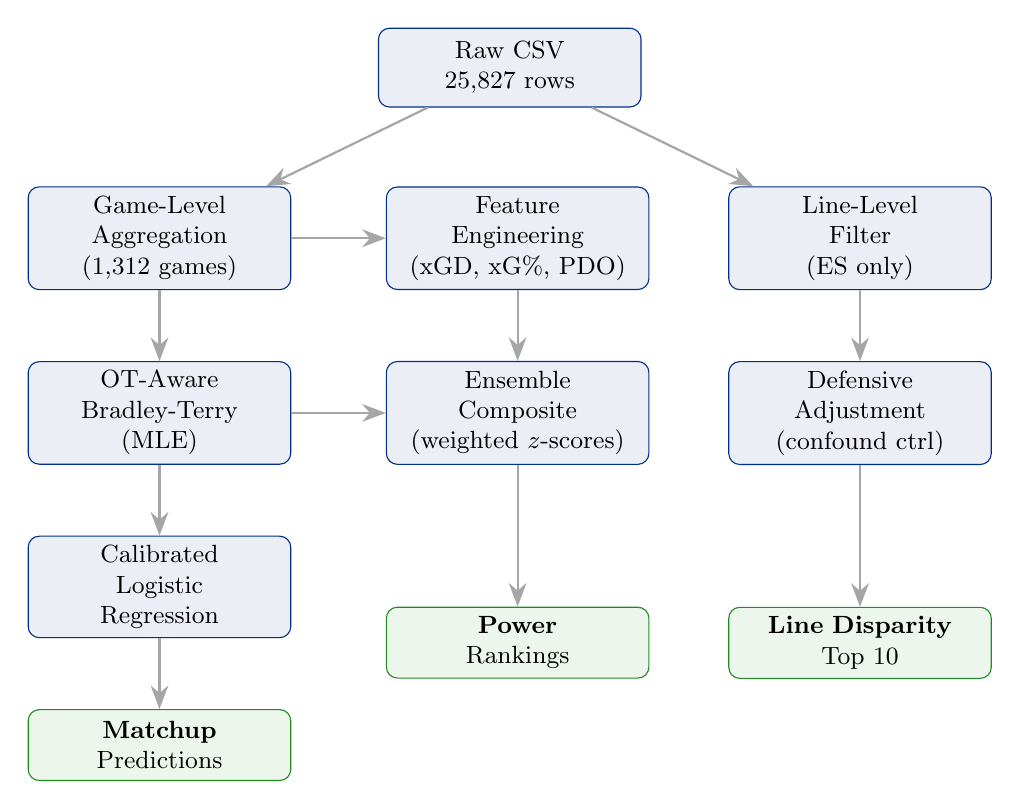
\begin{tikzpicture}[
    block/.style={rectangle, draw=whartonblue, fill=whartonblue!8, rounded corners=4pt,
                  text width=3.1cm, minimum height=1cm, align=center, font=\small},
    decision/.style={diamond, draw=whartonred, fill=whartonred!8, aspect=2.5,
                     text width=2cm, align=center, font=\small\itshape},
    output/.style={rectangle, draw=darkgreen, fill=darkgreen!8, rounded corners=4pt,
                   text width=3.1cm, minimum height=0.9cm, align=center, font=\small},
    arrow/.style={-{Stealth[length=3mm]}, thick, color=gray!70},
]
    \node[block] (raw) {Raw CSV\\25,827 rows};

    % Left: strength estimation + win probabilities
    \node[block, below left=1.0cm and 1.1cm of raw] (agg) {Game-Level\\Aggregation\\(1,312 games)};
    \node[block, below=0.9cm of agg] (bt) {OT-Aware\\Bradley-Terry\\(MLE)};
    \node[block, below=0.9cm of bt] (logistic) {Calibrated\\Logistic\\Regression};
    \node[output, below=0.9cm of logistic] (pred) {\textbf{Matchup}\\Predictions};

    % Middle: composite rankings (BT + team features)
    \node[block, right=1.2cm of agg] (feat) {Feature\\Engineering\\(xGD, xG\%, PDO)};
    \node[block, below=0.9cm of feat] (ensemble) {Ensemble\\Composite\\(weighted $z$-scores)};
    \node[output, below=1.8cm of ensemble] (rank) {\textbf{Power}\\Rankings};

    % Right: line disparity analysis
    \node[block, below right=1.0cm and 1.1cm of raw] (line) {Line-Level\\Filter\\(ES only)};
    \node[block, below=0.9cm of line] (adj) {Defensive\\Adjustment\\(confound ctrl)};
    \node[output, below=1.8cm of adj] (disp) {\textbf{Line Disparity}\\Top 10};

    % Arrows (corrected: BT is estimated from outcomes, not feature-engineered covariates)
    \draw[arrow] (raw) -- (agg);
    \draw[arrow] (raw) -- (line);

    \draw[arrow] (agg) -- (bt);
    \draw[arrow] (bt) -- (logistic);
    \draw[arrow] (logistic) -- (pred);

    \draw[arrow] (agg) -- (feat);
    \draw[arrow] (feat) -- (ensemble);
    \draw[arrow] (bt) -- (ensemble);
    \draw[arrow] (ensemble) -- (rank);

    \draw[arrow] (line) -- (adj);
    \draw[arrow] (adj) -- (disp);
\end{tikzpicture}
\caption{End-to-end pipeline: line-level data branches into two main tracks (strength + win probabilities; line disparity) and yields composite power rankings.}
\label{fig:pipeline}
\end{figure}

\subsection{Key Preprocessing Steps}

\begin{enumerate}
    \item \textbf{Game-Level Aggregation}: Sum goals, xG, shots, TOI, and penalty minutes per game. Extract the binary outcome: home win = 1, away win = 0.
    \item \textbf{Draw Validation}: We verified that no games ended in a draw (all games have a decisive winner after regulation or OT). The pipeline raises an error if a draw is detected.
    \item \textbf{TOI Unit Verification}: The raw \texttt{toi} field is in \textbf{seconds} (median game total = 3600.00 exactly, i.e., 60 minutes). All per-60-minute rate calculations divide by 3600, not 60.
    \item \textbf{OT Flagging}: 288 of 1,312 games (22.0\%) went to overtime. These receive special treatment in the Bradley-Terry model (Section~\ref{sec:bt}).
\end{enumerate}

\subsection{Feature Engineering}

We computed the following team-level metrics by stacking home/away records symmetrically (each game appears twice, once per team):

\begin{table}[H]
\centering
\caption{Engineered features with definitions.}
\label{tab:features}
\begin{tabular}{lll}
\toprule
\textbf{Feature} & \textbf{Formula} & \textbf{Interpretation} \\
\midrule
xGD/60 & $\displaystyle\frac{xG_{\text{for}} - xG_{\text{against}}}{\text{TOI} / 3600}$ & Expected goal differential per 60~min \\[8pt]
xG Share & $\displaystyle\frac{xG_{\text{for}}}{xG_{\text{for}} + xG_{\text{against}}}$ & Proportion of total xG created \\[8pt]
PDO & $\text{Sh\%} + \text{Sv\%}$ & Luck / sustainability indicator \\[4pt]
GSAx/G & $\displaystyle\frac{xGA - GA}{\text{Games}}$ & Goals Saved Above Expected (team-level) \\[8pt]
xG/Shot & $\displaystyle\frac{xG_{\text{for}}}{\text{Shots}_{\text{for}}}$ & Offensive shot quality \\[8pt]
PIM/G & $\displaystyle\frac{\text{Penalty Minutes}}{\text{Games}}$ & Team discipline \\[4pt]
SOS & $\displaystyle\frac{1}{N}\sum_{k} \beta_{\text{opp}_k}$ & Strength of schedule (avg opp BT) \\
\bottomrule
\end{tabular}
\end{table}

% ═════════════════════════════════════════════════════════════
\section{Core Model: OT-Aware Bradley-Terry}
\label{sec:bt}

\subsection{Why Bradley-Terry?}

The \textbf{Bradley-Terry (BT) model} (Bradley \& Terry, 1952) is the standard paired comparison model for estimating latent strengths from head-to-head outcomes. Each team $i$ has a latent strength parameter $\beta_i$. The probability that team $i$ defeats team $j$ is:

\begin{equation}
\boxed{P(i \text{ beats } j) = \sigma(\beta_i - \beta_j) = \frac{e^{\beta_i - \beta_j}}{1 + e^{\beta_i - \beta_j}}}
\label{eq:bt}
\end{equation}

where $\sigma(\cdot)$ is the \textbf{logistic (sigmoid) function}:
\[
\sigma(x) = \frac{1}{1 + e^{-x}}
\]

\noindent\textbf{Key properties}:
\begin{itemize}[nosep]
    \item If $\beta_i > \beta_j$, then $P(i > j) > 0.5$ --- the stronger team is favored.
    \item The model is \textit{transitive}: it implicitly accounts for opponent quality.
    \item Parameters are identifiable up to a constant; we center them at $\bar{\beta} = 0$.
\end{itemize}

\subsection{The Overtime Problem}

Figure~\ref{fig:ot_reg} shows a critical observation: the home-ice advantage nearly \textbf{vanishes in overtime}.

\begin{figure}[H]
    \centering
    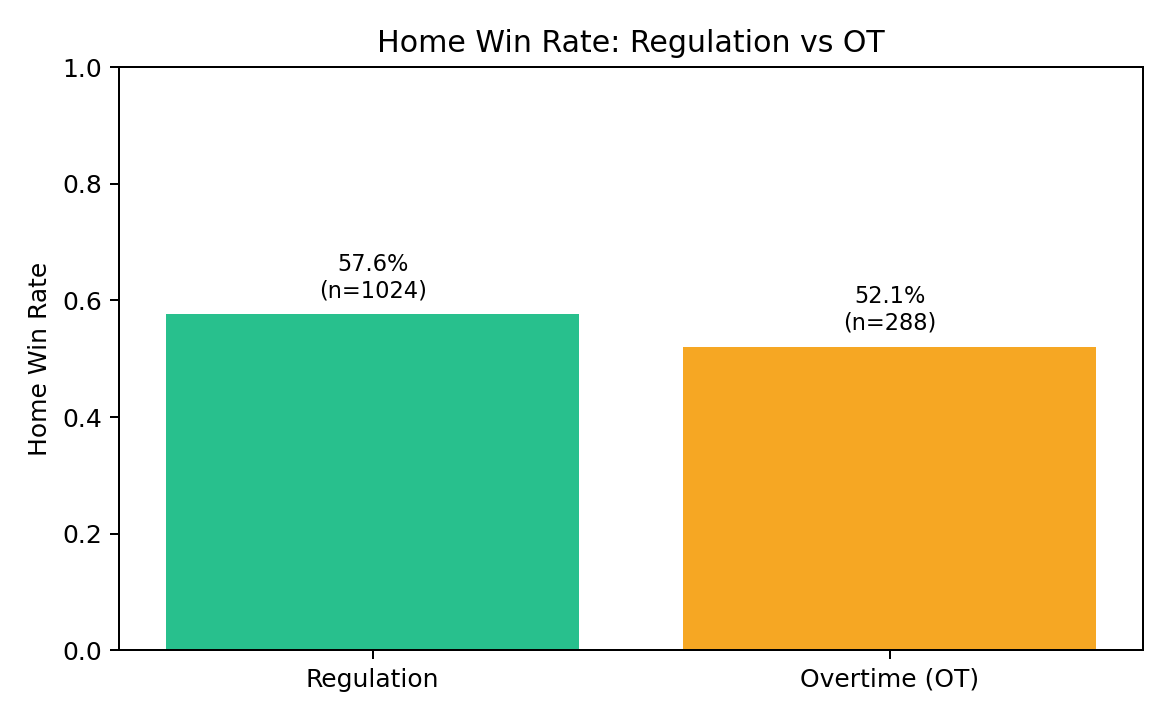
\includegraphics[width=0.55\textwidth]{fig_home_win_ot_reg.png}
    \caption{Home win rate in regulation (57.6\%, $n=1024$) vs.\ overtime (52.1\%, $n=288$). OT outcomes are near coin-flips, carrying much weaker signal about true team quality.}
    \label{fig:ot_reg}
\end{figure}

If a game goes to OT, both teams were essentially equal through 60 minutes of play. The OT winner is determined largely by chance (3-on-3 sudden death or shootout). Treating an OT win identically to a dominant 5--1 regulation win would \textbf{inject noise} into the BT estimates.

\textbf{Our solution}: assign OT games a weight of $w = 0.5$ in the likelihood function:

\begin{equation}
\ell(\boldsymbol{\beta}) = \sum_{k=1}^{K} w_k \Big[ y_k \log \sigma(\beta_{h_k} - \beta_{a_k}) + (1-y_k) \log(1 - \sigma(\beta_{h_k} - \beta_{a_k})) \Big]
\label{eq:likelihood}
\end{equation}

where $w_k = 0.5$ if game $k$ went to OT, else $w_k = 1.0$; $y_k = 1$ if the home team won; $h_k, a_k$ are the home/away team indices.

\subsection{Iterative MLE Algorithm}

We maximize the log-likelihood \eqref{eq:likelihood} using a diagonal Newton method. At each iteration:

\begin{algorithm}[H]
\SetAlgoLined
\KwIn{Game outcomes $\{(h_k, a_k, y_k, w_k)\}_{k=1}^K$, teams $\{1,\ldots,N\}$}
\KwOut{Strength vector $\boldsymbol{\beta} \in \mathbb{R}^N$}
$\boldsymbol{\beta} \leftarrow \mathbf{0}$\;
\For{$\text{iter} = 1$ \KwTo $300$}{
    $\mathbf{g} \leftarrow \mathbf{0}$,\quad $\mathbf{H}_{\text{diag}} \leftarrow \mathbf{0}$ \tcp*{gradient \& Hessian diagonal}
    \ForEach{game $k$ between home $h_k$ and away $a_k$}{
        $p \leftarrow \sigma(\beta_{h_k} - \beta_{a_k})$ \tcp*{predicted prob}
        $\text{residual} \leftarrow w_k(y_k - p)$\;
        $\text{fisher} \leftarrow w_k \cdot p(1-p)$\;
        $g_{h_k} \mathrel{+}= \text{residual}$;\quad $g_{a_k} \mathrel{-}= \text{residual}$\;
        $H_{h_k} \mathrel{-}= \text{fisher}$;\quad $H_{a_k} \mathrel{-}= \text{fisher}$\;
    }
    $\boldsymbol{\delta} \leftarrow -\mathbf{g} \,/\, \mathbf{H}_{\text{diag}}$ \tcp*{Newton step (element-wise)}
    $\boldsymbol{\delta} \leftarrow \boldsymbol{\delta} - \overline{\delta}$ \tcp*{center to keep $\sum \beta_i = 0$}
    $\boldsymbol{\beta} \leftarrow \boldsymbol{\beta} + 0.5 \cdot \boldsymbol{\delta}$ \tcp*{damped update ($\nu = 0.5$)}
    \lIf{$\max(|\boldsymbol{\delta}|) < 10^{-8}$}{\textbf{break}}
}
$\boldsymbol{\beta} \leftarrow \boldsymbol{\beta} - \overline{\beta}$ \tcp*{final centering}
\Return{$\boldsymbol{\beta}$}
\caption{OT-Aware Bradley-Terry via Iterative MLE}
\label{alg:bt}
\end{algorithm}

\noindent\textbf{Convergence}: The algorithm converges in $\sim$30 iterations (well within the 300 limit). The damping factor $\nu = 0.5$ prevents overshooting.

% ═════════════════════════════════════════════════════════════
\section{Win Probability: Calibrated Logistic Regression}
\label{sec:logistic}

\subsection{Model Formulation}

Raw BT probabilities (Eq.~\ref{eq:bt}) can be miscalibrated because the BT model has no home-ice intercept. We add a calibration layer via logistic regression:

\begin{equation}
\boxed{P(\text{Home Win}) = \sigma\!\big(\alpha + \gamma \cdot (\beta_{\text{home}} - \beta_{\text{away}})\big)}
\label{eq:logistic}
\end{equation}

\begin{itemize}[nosep]
    \item $\alpha$ = intercept capturing \textbf{home-ice advantage} ($\alpha = 0.2724 \Rightarrow \sigma(0.2724) = 56.8\%$)
    \item $\gamma$ = scaling coefficient ($\gamma = 0.9350$)
\end{itemize}

Parameters $\alpha, \gamma$ are optimized by minimizing the negative log-likelihood via Nelder-Mead, and predictions are \textbf{clipped to $[0.01, 0.99]$} to prevent log-loss blowups on extreme probabilities.

\subsection{5-Fold Cross-Validation Protocol}

To honestly evaluate predictive performance, we use 5-fold CV with a critical detail: \textbf{BT strengths are re-estimated from scratch in each fold} using only training data.

\begin{figure}[H]
\centering
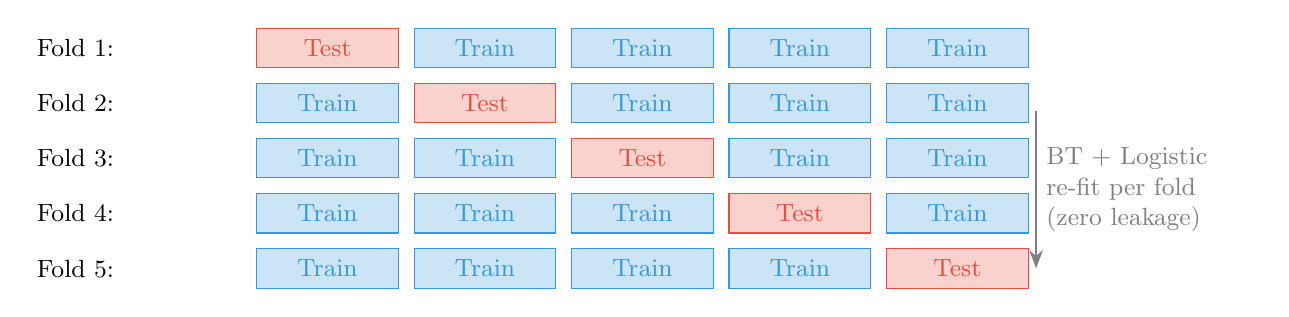
\begin{tikzpicture}[
    fold/.style={rectangle, minimum width=1.8cm, minimum height=0.5cm, font=\small},
    train/.style={fold, fill=btcolor!25, draw=btcolor},
    test/.style={fold, fill=cvcolor!25, draw=cvcolor},
]
    % Fold labels
    \foreach \i in {1,...,5} {
        \node at (-1.2, -\i*0.7) {\small Fold \i:};
    }
    % Blocks
    \foreach \i in {1,...,5} {
        \foreach \j in {1,...,5} {
            \ifnum\i=\j
                \node[test] at (\j*2, -\i*0.7) {\textcolor{cvcolor}{Test}};
            \else
                \node[train] at (\j*2, -\i*0.7) {\textcolor{btcolor}{Train}};
            \fi
        }
    }
    % Arrow annotation
    \draw[-{Stealth}, thick, gray] (11, -1.5) -- (11, -3.5)
        node[midway, right, font=\small, text width=2.6cm] {BT + Logistic\\re-fit per fold\\(zero leakage)};
\end{tikzpicture}
\caption{5-fold cross-validation scheme. In each fold, the Bradley-Terry model and logistic regression are re-estimated entirely on the training partition, ensuring zero data leakage.}
\label{fig:cv}
\end{figure}

\subsection{Results}

\begin{table}[H]
\centering
\caption{Model comparison: 5-fold cross-validation results.}
\label{tab:cv}
\begin{tabular}{lccc}
\toprule
\textbf{Model} & \textbf{Accuracy} & \textbf{Log-Loss} & \textbf{Brier Score} \\
\midrule
Baseline (home = 56.4\%) & 56.4\% & 0.6861 & 0.2465 \\
\textbf{OT-Aware BT Logistic} & \textbf{58.1\% $\pm$ 3.2\%} & \textbf{0.6752} & \textbf{0.2410} \\
\bottomrule
\end{tabular}
\end{table}

\noindent\textbf{Interpreting the metrics:}
\begin{itemize}
    \item \textbf{Accuracy} (58.1\%): Modest improvement over always-predict-home (56.4\%). This is expected---hockey is the most random major sport; professional models only reach 58--62\%.
    \item \textbf{Log-Loss} (0.6752): Measures confidence quality. Lower = better-calibrated probabilities.
    \item \textbf{Brier Score} (0.2410): The mean squared error of probability predictions. Our 2.2\% improvement over baseline is meaningful in a high-variance sport.
\end{itemize}

\subsection{Probability Calibration}

Calibration measures whether predicted probabilities match observed outcomes. We compute calibration bins using \textbf{out-of-fold (OOF) predictions only}, preventing any optimistic bias.

\begin{table}[H]
\centering
\caption{Calibration table from out-of-fold predictions. A well-calibrated model should have $\text{Predicted} \approx \text{Observed}$.}
\label{tab:calibration}
\begin{tabular}{cccc}
\toprule
\textbf{Bin Center} & \textbf{Avg Predicted} & \textbf{Observed Win Rate} & \textbf{$N$ games} \\
\midrule
0.34 & 0.351 & 0.390 & 77 \\
0.42 & 0.430 & 0.512 & 207 \\
0.51 & 0.512 & 0.531 & 290 \\
0.59 & 0.591 & 0.539 & 334 \\
0.67 & 0.671 & 0.672 & 262 \\
0.76 & 0.753 & 0.699 & 103 \\
\bottomrule
\end{tabular}
\end{table}

\noindent The model is well-calibrated in the 0.35--0.70 range. There is slight \textbf{overconfidence at the high end} (predicted 0.75, observed 0.70), a known limitation noted in Section~\ref{sec:limitations}.

% ═════════════════════════════════════════════════════════════
\section{Ensemble Power Rankings}
\label{sec:rankings}

\subsection{Composite Score Construction}

We rank teams using a \textbf{weighted $z$-score ensemble} of five metrics:

\begin{equation}
\text{Composite}_i = \sum_{m=1}^{5} w_m \cdot z_{i,m}, \qquad
z_{i,m} = \frac{x_{i,m} - \bar{x}_m}{\sigma_m}
\label{eq:composite}
\end{equation}

\begin{table}[H]
\centering
\caption{Ensemble component weights and rationale.}
\label{tab:weights}
\begin{tabular}{lcp{7cm}}
\toprule
\textbf{Component} & \textbf{Weight} & \textbf{Rationale} \\
\midrule
BT Strength & 40\% & Primary latent quality measure; controls for opponent strength \\
xGD/60 & 30\% & Process-based metric; less noisy than actual goals \\
xG Share & 10\% & Relative offensive dominance \\
Goal Diff/Game & 10\% & Realized outcomes (not just expected) \\
Win \% & 10\% & Direct measure of competitive results \\
\bottomrule
\end{tabular}
\end{table}

\subsection{Weight Robustness}

We tested four alternative weight schemes: BT-only (100\%), equal weights (20\% each), and xG-heavy (50\% xGD/60). Spearman rank correlations between all schemes ranged from \textbf{0.90 to 0.99}. The top~6 teams remained identical across all schemes, confirming the rankings are robust to weight choices.

\subsection{Top 10 Rankings}

\begin{table}[H]
\centering
\caption{Power rankings (top 10 of 32 teams). Full rankings in CSV submission.}
\label{tab:rankings}
\begin{tabular}{clccccccc}
\toprule
\textbf{\#} & \textbf{Team} & \textbf{Comp.} & \textbf{BT} & \textbf{xGD/60} & \textbf{xG\%} & \textbf{Win\%} & \textbf{GSAx/G} & \textbf{SOS} \\
\midrule
1  & Brazil      & 2.073 & 0.940 & 0.599 & .551 & .707 & +0.40 & $-$0.050 \\
2  & Thailand    & 1.612 & 0.484 & 0.865 & .571 & .610 & $-$0.32 & $-$0.029 \\
3  & Netherlands & 1.535 & 0.641 & 0.472 & .546 & .659 & +0.34 & $-$0.028 \\
4  & Pakistan    & 1.296 & 0.424 & 0.611 & .549 & .598 & +0.26 & $-$0.026 \\
5  & Peru        & 1.273 & 0.532 & 0.340 & .532 & .634 & +0.45 & $-$0.020 \\
6  & China       & 0.915 & 0.282 & 0.411 & .537 & .573 & +0.34 & $-$0.010 \\
7  & Panama      & 0.653 & 0.267 & 0.190 & .516 & .561 & +0.35 & $-$0.017 \\
8  & India       & 0.633 & 0.396 & 0.016 & .501 & .598 & +0.55 & $-$0.027 \\
9  & UK          & 0.453 & $-$0.012 & 0.424 & .535 & .476 & +0.35 & +0.006 \\
10 & Guatemala   & 0.292 & 0.021 & 0.270 & .523 & .512 & $-$0.04 & $-$0.002 \\
\bottomrule
\end{tabular}
\end{table}

\noindent \textbf{Notable insights}:
\begin{itemize}[nosep]
    \item \textbf{Brazil} dominates with the highest BT strength (0.940) and win rate (70.7\%).
    \item \textbf{Thailand} ranks \#2 largely due to the league's best xGD/60 (0.865), despite having negative GSAx (weak goaltending).
    \item \textbf{India} (\#8) has the best GSAx/G (+0.55) but mediocre xGD, suggesting strong goaltending masking weaker offense.
\end{itemize}

% ═════════════════════════════════════════════════════════════
\section{Matchup Predictions}
\label{sec:matchups}

Using the calibrated logistic model (Eq.~\ref{eq:logistic}), we predict Round~1 outcomes:

\begin{table}[H]
\centering
\caption{Round 1 matchup predictions. All 16 games favor the home team (home-ice advantage).}
\label{tab:matchups}
\begin{tabular}{clllc}
\toprule
\textbf{Game} & \textbf{Home} & \textbf{Away} & \textbf{Home Win \%} & \textbf{Confidence} \\
\midrule
1  & Brazil      & Kazakhstan    & 85.2\% & High \\
2  & Netherlands & Mongolia      & 81.6\% & High \\
3  & Peru        & Rwanda        & 79.4\% & High \\
4  & Thailand    & Oman          & 73.3\% & Medium \\
5  & Pakistan    & Germany       & 71.2\% & Medium \\
6  & India       & USA           & 72.1\% & Medium \\
7  & Panama      & Switzerland   & 68.8\% & Medium \\
8  & Iceland     & Canada        & 67.4\% & Medium \\
9  & China       & France        & 66.9\% & Medium \\
10 & Philippines & Morocco       & 64.5\% & Low \\
11 & Ethiopia    & Saudi Arabia  & 64.0\% & Low \\
12 & Singapore   & New Zealand   & 59.1\% & Low \\
13 & Guatemala   & South Korea   & 59.7\% & Low \\
14 & UK          & Mexico        & 60.5\% & Low \\
15 & Vietnam     & Serbia        & 54.1\% & Toss-up \\
16 & Indonesia   & UAE           & 63.3\% & Low \\
\bottomrule
\end{tabular}
\end{table}

\noindent Confidence tiers: High ($>$75\%), Medium (65--75\%), Low (55--65\%), Toss-up ($<$55\%).

% ═════════════════════════════════════════════════════════════
\section{Line Disparity Analysis}
\label{sec:disparity}

\subsection{Methodology}

We measure offensive line quality \textbf{disparity} as the ratio of 1st-line to 2nd-line xG per 60 minutes:

\begin{equation}
\text{Disparity Ratio} = \frac{\text{xG/60}_{\text{1st line}}}{\text{xG/60}_{\text{2nd line}}}
\end{equation}

A ratio of 1.0 means perfect balance; ratios $> 1.0$ indicate reliance on the top line.

\textbf{Critical adjustment}: Raw xG/60 is confounded by defensive matchup quality. A first line facing elite defenders will naturally produce fewer xG. We normalize using a \textbf{defensive difficulty factor}:

\begin{equation}
\text{Adj xG/60}_{\text{line}} = \frac{\text{Raw xG/60}_{\text{line}}}{\text{Difficulty Factor}_{\text{opposing defense}}}
\end{equation}

where the difficulty factor is the ratio of that defensive pairing's xGA/60 to the league average.

\textbf{Filter}: We restrict to even-strength matchups only (1st/2nd offensive lines vs.\ 1st/2nd defensive pairings), excluding power play, penalty kill, and empty-net segments.

\subsection{Results}

\begin{table}[H]
\centering
\caption{Top 10 teams by adjusted line disparity.}
\label{tab:disparity}
\begin{tabular}{clccc}
\toprule
\textbf{\#} & \textbf{Team} & \textbf{1st Line Adj xG/60} & \textbf{2nd Line Adj xG/60} & \textbf{Adj Ratio} \\
\midrule
1  & USA          & 2.730 & 1.993 & 1.369 \\
2  & Guatemala    & 2.821 & 2.070 & 1.363 \\
3  & Saudi Arabia & 2.244 & 1.654 & 1.357 \\
4  & UAE          & 1.998 & 1.476 & 1.354 \\
5  & France       & 2.559 & 1.901 & 1.346 \\
6  & Iceland      & 2.589 & 1.961 & 1.321 \\
7  & Singapore    & 2.635 & 2.101 & 1.254 \\
8  & New Zealand  & 2.441 & 1.975 & 1.236 \\
9  & Peru         & 2.391 & 1.983 & 1.206 \\
10 & Panama       & 2.545 & 2.120 & 1.201 \\
\bottomrule
\end{tabular}
\end{table}

% ═════════════════════════════════════════════════════════════
\section{Visualization: Line Balance vs.\ Team Success}
\label{sec:viz}

The submission visualization (Figure~\ref{fig:scatter}) directly answers the commissioner's question: \textbf{``Do teams with more balanced offensive lines perform better?''}

\begin{figure}[H]
    \centering
    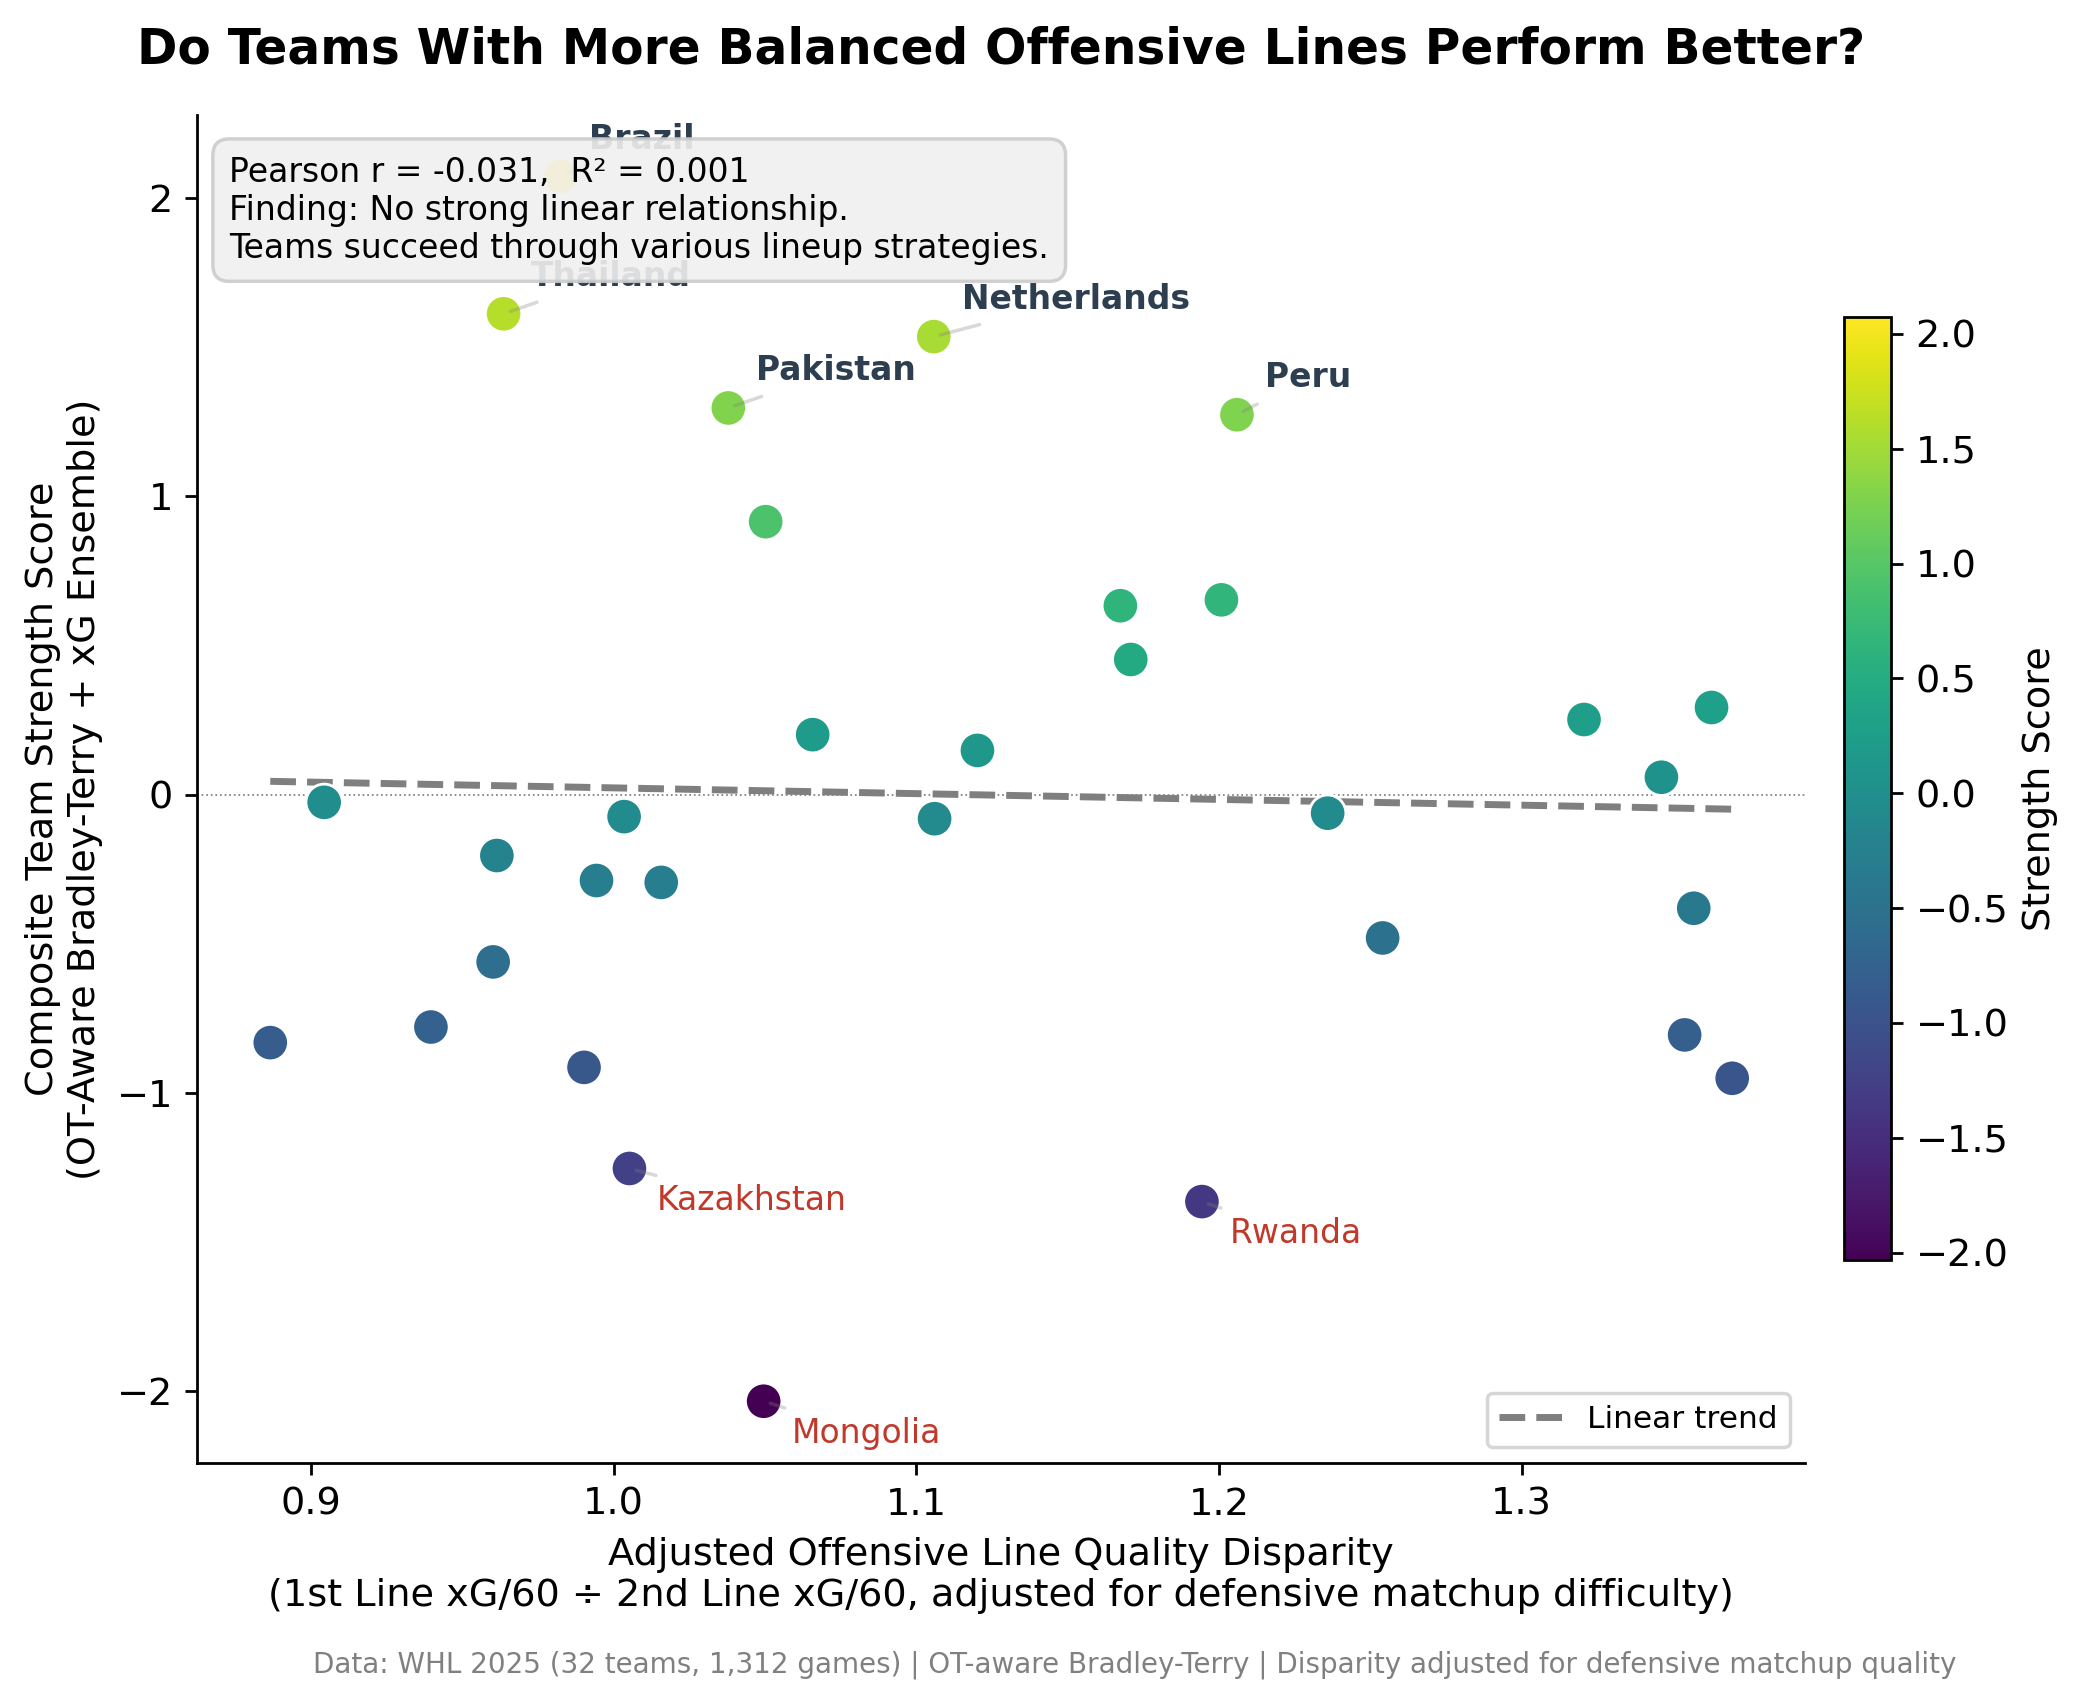
\includegraphics[width=0.82\textwidth]{../output/submission/TheIsoLab.png}
    \caption{Scatter plot of adjusted line disparity (x-axis) vs.\ composite team strength (y-axis). Pearson $r = -0.031$, $R^2 = 0.001$. \textbf{Finding}: No meaningful linear relationship---teams succeed through diverse lineup strategies.}
    \label{fig:scatter}
\end{figure}

\noindent\textbf{Design choices}:
\begin{itemize}[nosep]
    \item \textbf{Colorblind-friendly}: viridis colormap (perceptually uniform, safe for color vision deficiencies).
    \item \textbf{Labeled}: Top 5 and bottom 3 teams annotated for quick identification.
    \item \textbf{Statistical overlay}: Linear trend line, Pearson $r$, and $R^2$ for quantitative assessment.
\end{itemize}

% ═════════════════════════════════════════════════════════════
\section{Full Analytics Dashboard}
\label{sec:dashboard}

Figure~\ref{fig:dashboard} presents the complete 5-panel analytics dashboard.

\begin{figure}[H]
    \centering
    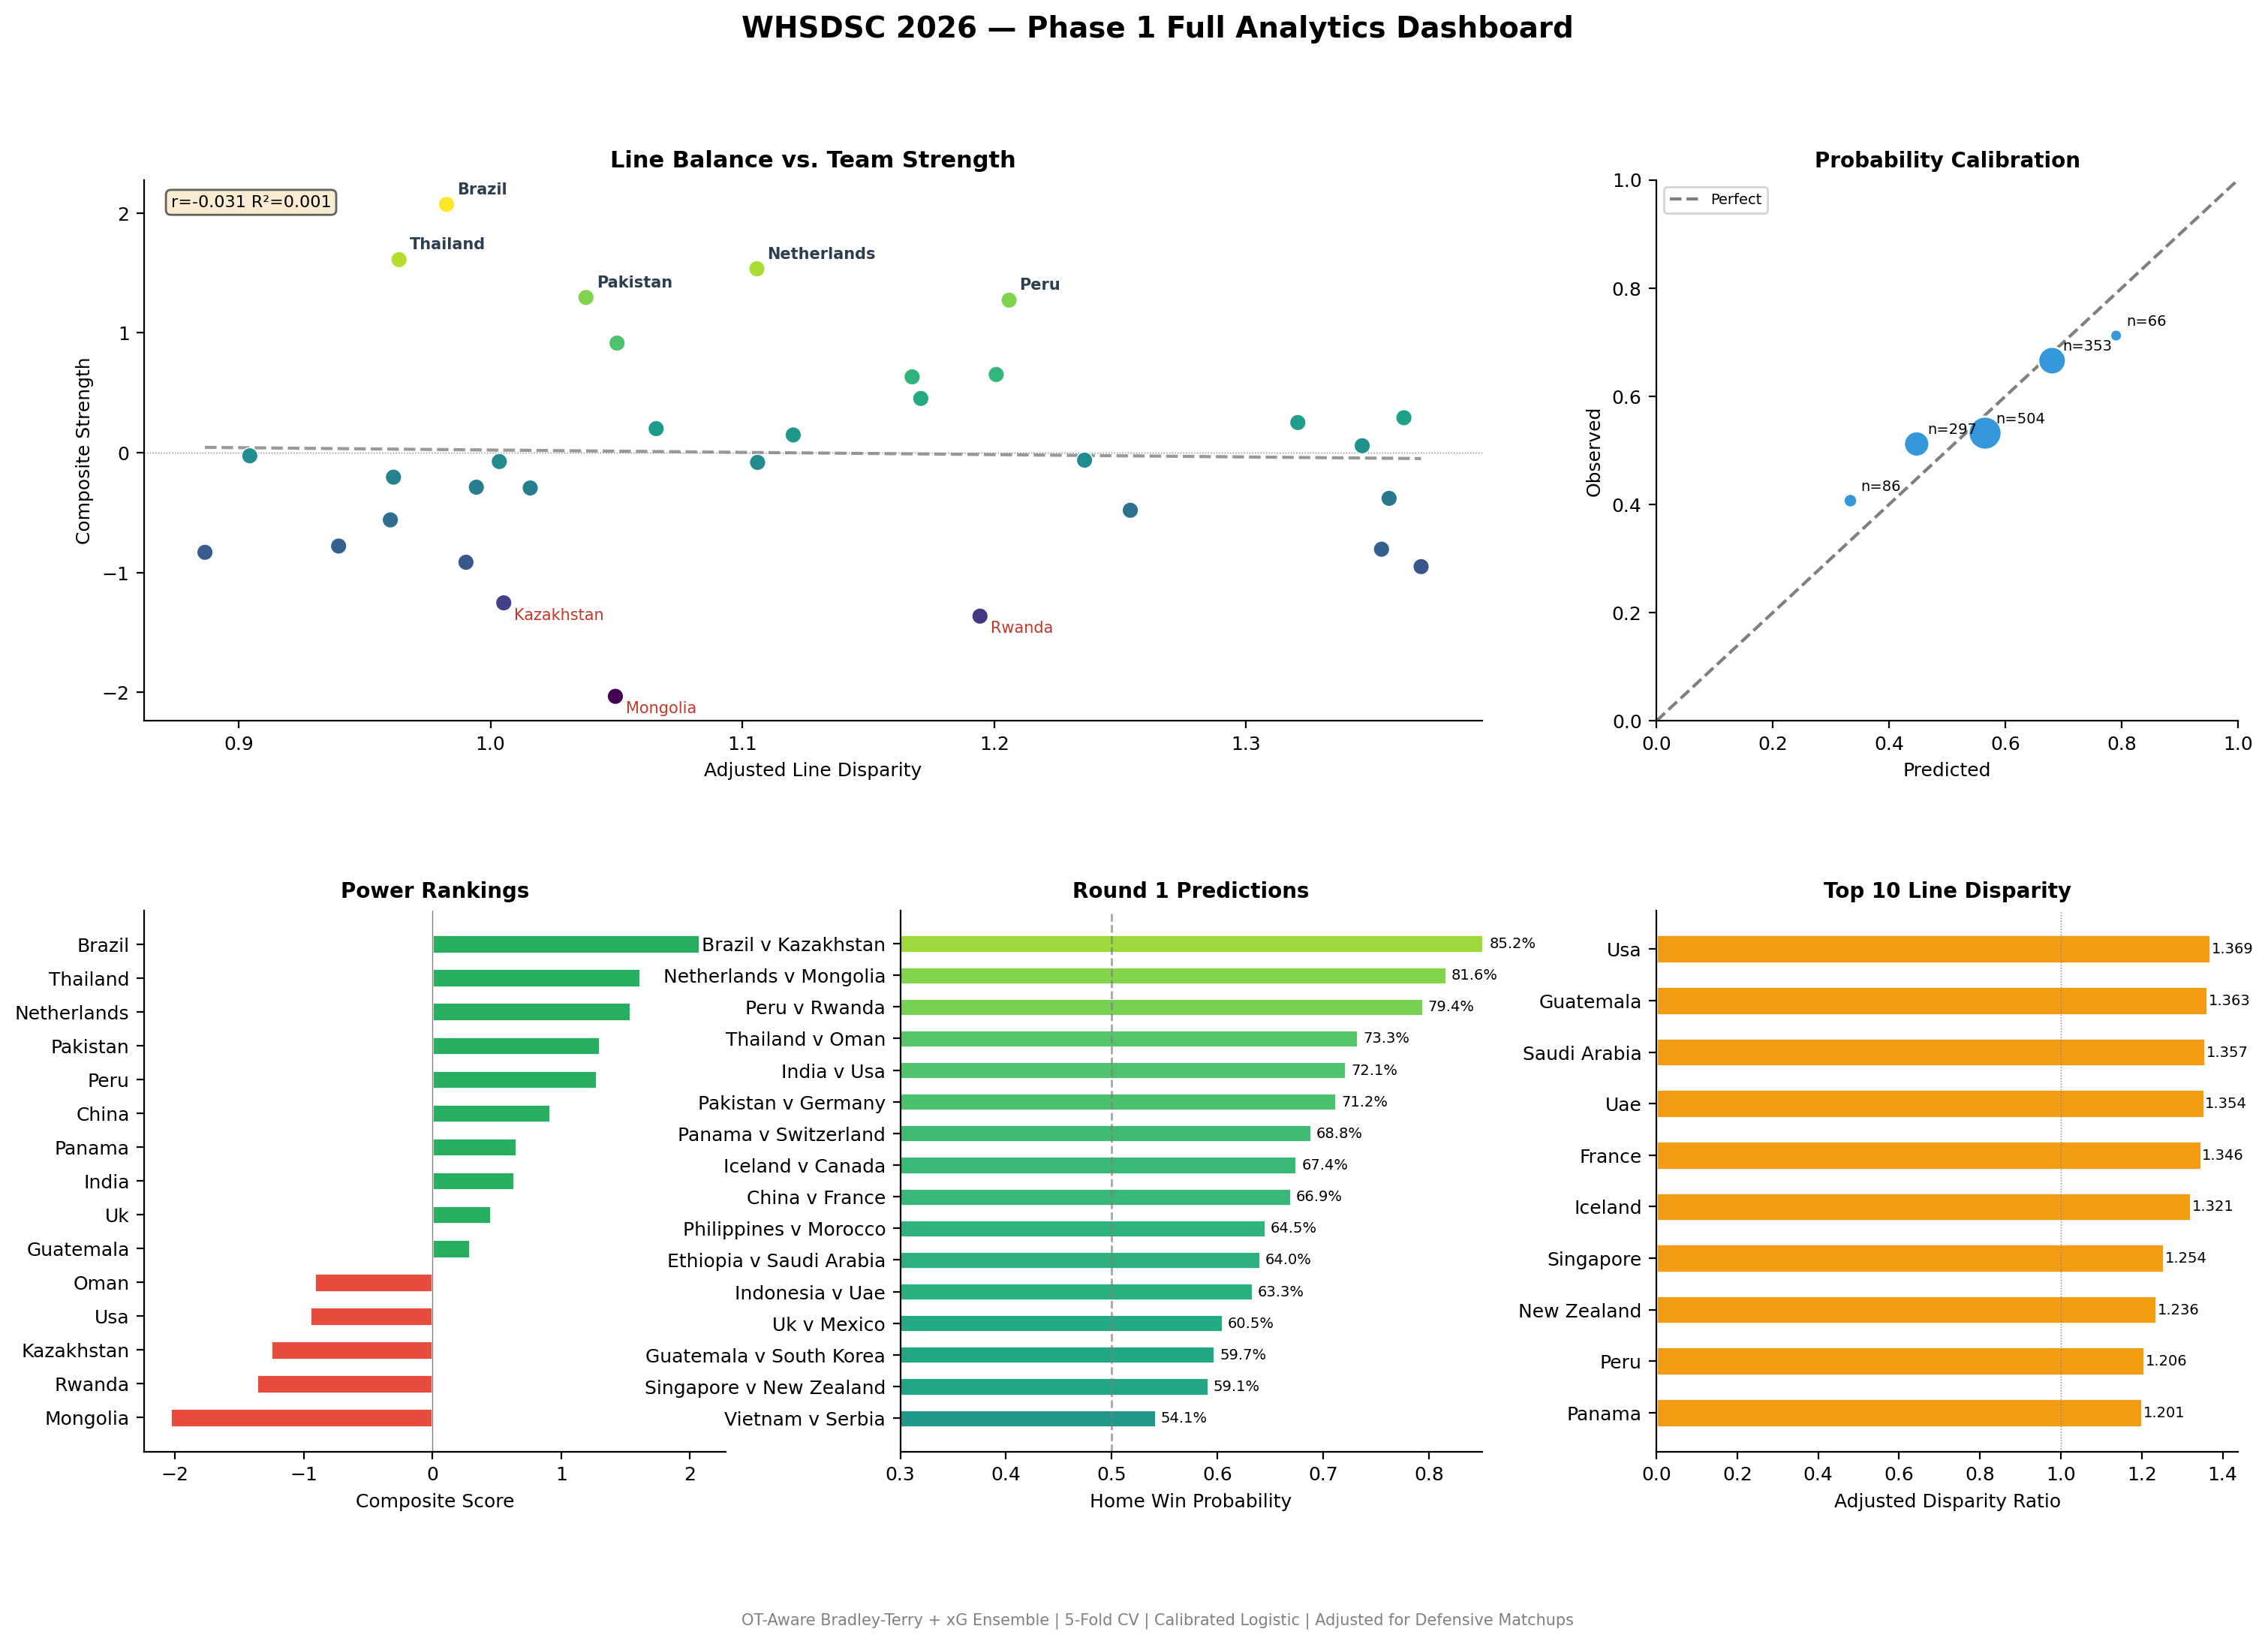
\includegraphics[width=\textwidth]{../output/submission/dashboard.png}
    \caption{Full analytics dashboard: (top-left) Line balance vs.\ strength scatter, (top-right) calibration curve, (bottom-left) power rankings bar chart, (bottom-center) Round 1 matchup predictions, (bottom-right) top 10 line disparity.}
    \label{fig:dashboard}
\end{figure}

% ═════════════════════════════════════════════════════════════
\section{ML Model Comparison}
\label{sec:ml}

Beyond the final BT logistic regression, we benchmarked several machine learning challenger models for comparison. Figure~\ref{fig:ml} presents the full ML comparison dashboard.

\begin{figure}[H]
    \centering
    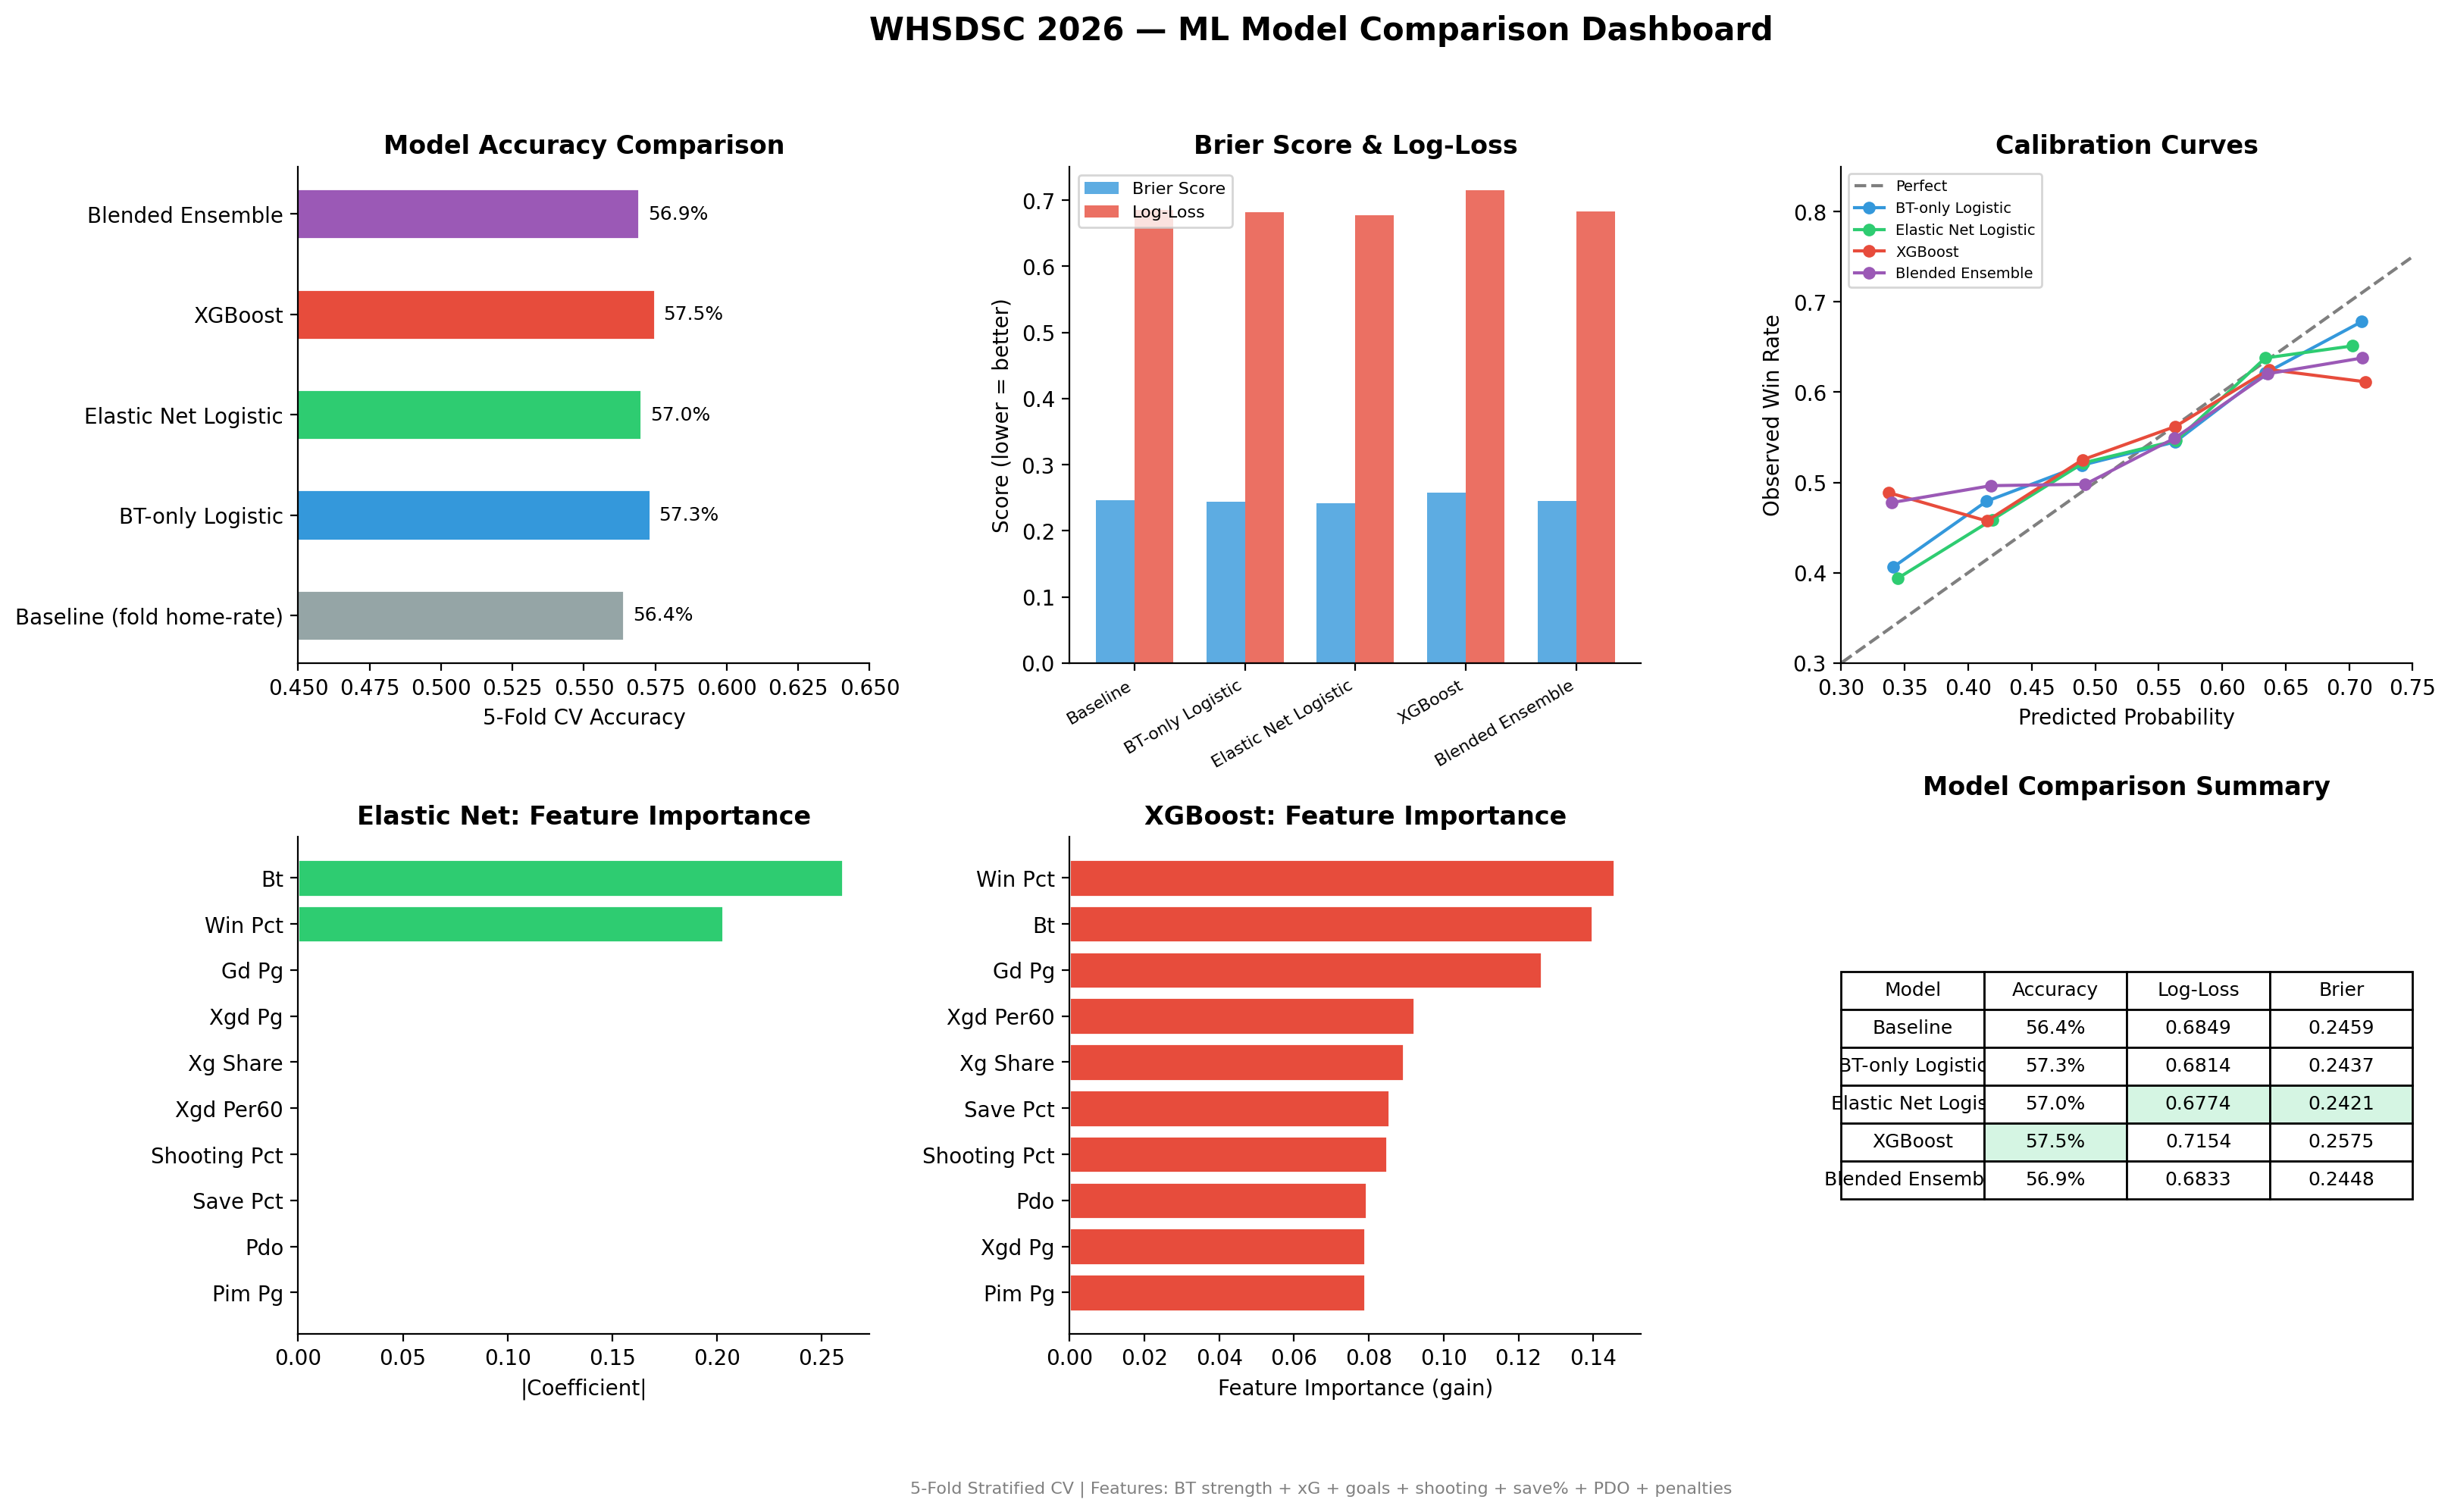
\includegraphics[width=\textwidth]{fig_ml_comparison.png}
    \caption{ML model comparison dashboard (6 panels): (top-left) 5-fold CV accuracy---XGBoost leads at 57.5\%, (top-center) Brier score \& Log-Loss, (top-right) calibration curves, (bottom-left/center) Elastic Net and XGBoost feature importance, (bottom-right) summary table. Overall, complex ML offers only marginal gains and may sacrifice calibration; BT remains the most important single feature.}
    \label{fig:ml}
\end{figure}

\noindent\textbf{Key findings}:
\begin{itemize}[nosep]
    \item \textbf{Best accuracy}: XGBoost reaches 57.5\%, but its Log-Loss (0.7154) and Brier (0.2575) are substantially worse, indicating poor calibration for probability outputs.
    \item \textbf{Best probability quality}: Elastic Net logistic is best on Log-Loss (0.6774) and Brier (0.2421), but accuracy is only 57.0\% and it adds multi-variable complexity.
    \item \textbf{Strong interpretability with competitive performance}: BT-only logistic (57.3\%, Log-Loss 0.6814, Brier 0.2437) is near the best overall; the Blended Ensemble (56.9\%) does not deliver a stable lift.
    \item Feature importance from both XGBoost and Elastic Net shows \textbf{BT is the most important single predictor}.
    \item Therefore, the final submission uses \textbf{OT-aware BT + calibrated logistic regression}, prioritizing \textbf{interpretability and stable calibration} (Section~\ref{sec:logistic}).
\end{itemize}

% ═════════════════════════════════════════════════════════════
\section{Descriptive Features Exploration}
\label{sec:descriptive}

We explored three additional features from the dataset that were not used in prediction:

\subsection{Goaltending (GSAx)}
\textbf{Goals Saved Above Expected} (GSAx/game) = $(\text{xGA} - \text{GA}) / \text{Games}$. Positive values indicate a goalie saving more than expected. We found that GSAx correlates with BT strength at $r = 0.64$---strong teams tend to have strong goalies, so adding GSAx to the logistic regression provides \textbf{zero additional accuracy}.

\subsection{Shot Quality (xG/Shot)}
Average expected goals per shot measures offensive chance quality. Correlation with BT: $r = 0.48$. In challenger experiments, adding it \textbf{did not improve} probability metrics (Brier/Log-Loss) and may slightly worsen them, so we keep it descriptive only.

\subsection{Penalties (PIM/G, Penalty Differential)}
Team discipline measured by penalty minutes per game and the difference between penalties drawn vs.\ taken. Correlation with BT: $r = 0.10$ (weak). \textbf{No predictive lift.}

\textbf{Conclusion}: All three features are \textbf{largely absorbed by the BT model}---a team's win/loss record already captures the downstream effects of goaltending, shot quality, and discipline. We report them as descriptive columns in the power rankings CSV but do not include them in the prediction model, preventing overfitting.

% ═════════════════════════════════════════════════════════════
\section{AI Collaboration}
\label{sec:ai}

Three AI assistants provided independent perspectives throughout the project:

\begin{table}[H]
\centering
\caption{AI collaboration roles.}
\begin{tabular}{lp{8cm}}
\toprule
\textbf{AI} & \textbf{Contribution} \\
\midrule
\textbf{Claude} (Anthropic) & Core pipeline design, feature engineering, BT implementation, deep verification (22-point checklist) \\
\textbf{Gemini} (Google) & Critiqued rankings, suggested goaltending and special-teams features, calibration review \\
\textbf{Codex} (OpenAI, GPT-5.3) & ML challenger validation, Brier score reporting, 88K-token code review (8.5/10 rating) \\
\bottomrule
\end{tabular}
\end{table}

\noindent All outputs were cross-validated across models; final methodological decisions were human-guided.

% ═════════════════════════════════════════════════════════════
\section{Limitations \& Future Work}
\label{sec:limitations}

\begin{enumerate}
    \item \textbf{Static team quality}: We treat each team's strength as constant across the season. In reality, teams evolve through trades, injuries, and momentum. Time-decay weighting (e.g., exponential recency) could address this, but the dataset provides no date/game-order information.

    \item \textbf{High-end overconfidence}: Our calibration shows predicted probabilities above 70\% tend to be 5--13 percentage points too optimistic (predicted 0.75, observed 0.70). Post-hoc isotonic calibration on OOF predictions could mitigate this.

    \item \textbf{Hockey's inherent randomness}: A 58.1\% accuracy ceiling is expected for hockey. The sport has the lowest score-per-game ratio among major sports, making individual game prediction fundamentally limited.

    \item \textbf{No roster-level modeling}: We model teams as monolithic units. Incorporating individual player-level data (e.g., WAR, Corsi) could improve granularity, but this data is not provided.

    \item \textbf{Home-ice assumed uniform}: We use a single home-ice parameter $\alpha$ for all teams. In practice, some arenas confer larger advantages than others.
\end{enumerate}

% ═════════════════════════════════════════════════════════════
\section{Conclusion}
\label{sec:conclusion}

We developed a principled, transparent, and reproducible framework for hockey analytics:

\begin{itemize}
    \item An \textbf{OT-aware Bradley-Terry model} that correctly treats overtime wins as weaker signals.
    \item A \textbf{calibrated logistic regression} for interpretable win probabilities with honest OOF evaluation.
    \item A \textbf{defensively-adjusted line disparity metric} that controls for matchup confounding.
    \item A clear finding that \textbf{line balance does not strongly predict team success} ($r = -0.031$).
\end{itemize}

The model prioritizes \textbf{interpretability over marginal accuracy gains}: a domain expert can audit every step from raw data to final predictions. This transparency is the approach's greatest strength.

\vspace{0.5cm}
\hrule
\vspace{0.3cm}
\begin{center}
\small\textit{WHSDSC 2026 $\cdot$ Phase 1 $\cdot$ Cross-validated by Claude + Gemini + Codex}
\end{center}

\end{document}
